% Created 2013-05-29 Wed 23:26
\documentclass[11pt]{article}
\usepackage[utf8]{inputenc}
\usepackage[T1]{fontenc}
\usepackage{fixltx2e}
\usepackage{graphicx}
\usepackage{longtable}
\usepackage{float}
\usepackage{wrapfig}
\usepackage{soul}
\usepackage{textcomp}
\usepackage{marvosym}
\usepackage{wasysym}
\usepackage{latexsym}
\usepackage{amssymb}
\usepackage{amstext}
\usepackage{hyperref}
\tolerance=1000
\author{Hongbo Zhang}
\date{\today}
\title{Getting started}
\hypersetup{
  pdfkeywords={},
  pdfsubject={},
  pdfcreator={Emacs 23.3.50.1 (Org mode 8.0.3)}}
\begin{document}

\maketitle
\tableofcontents

The following post assumes the reader is already familiar with OCaml.
If you are not familiar with OCaml, \url{http://ocaml.org/} is recommended
for you to learn.


\section{Installation}
\label{sec-1}
see \href{install.org}{Installation}

\section{What language does Fan speak?}
\label{sec-2}

Fan speaks OCaml natively, plus a few addons. 

There are some minor differences between Fan's concrete syntax and
OCaml though, the major differences is that Fan is more strict than
OCaml.

Three particular points:
\begin{enumerate}
\item Parens are necessary for tuples
\begin{verbatim}
(** illegal *)
a,b 
let a,b = f in
    body
\end{verbatim}

\begin{verbatim}
(** correct syntax *)
(a,b )
let (a,b) = f in
    body
\end{verbatim}
\item Parens or "begin" "end" necessary for semis
\begin{verbatim}
(* illegal *)
print_endline "a"; print_endline "b"
\end{verbatim}
\begin{verbatim}
(** correct *)
(print_endline "a"; print_endline "b")
begin print_endline "a"; print_endline "b" end
\end{verbatim}
\item First vertical bar is necessary for algebraic data type, pattern
match.
\begin{verbatim}
(** illegal *)
type u = A | B
let f = function
    A -> "a"
  | B -> "b"
let f =
  match c with
    A -> "a"
  | B -> "b"
\end{verbatim}

\begin{verbatim}
(** correct *)
type u =
  | A
  | B 

let f = function
  | A -> "a"
  | B -> "b" 

let f =
  match c with
  | A -> "a"
  | B -> "b"
\end{verbatim}
\item \$ is a reserved operator, please don't take it as a function.
\end{enumerate}

\section{Compiing with Fan}
\label{sec-3}

\subsection{Hello world \label{hello}}
\label{sec-3-1}
Create a file \href{code/hello.ml}{hello.ml} as follows:

\begin{verbatim}
print_endline "hell, Fan"
\end{verbatim}

The compile is quite simple, make sure \texttt{fan.byte} or \texttt{fan.native} is
in your search path.

\begin{verbatim}
$ ocamlc -pp 'fan.native' hello.ml -o test
$ ./test
\end{verbatim}

As you may notice, adding \textasciitilde{}-pp 'fan.native'\textasciitilde{} flag is enough to
switching to Fan. Using \texttt{fan.byte} or \texttt{fan.native} is up to you,
for the time being, only the performance matters here. So,
compiling with the following command line does also work.

\begin{verbatim}
$ ocamlc -pp 'fan.native' hello.ml -o test
\end{verbatim}
\subsection{First class lexer}
\label{sec-3-2}

Writing hello world is not very interesting, for the following
example, we show you how DDSL fits into Fan. Suppose we want to
write a lexical analyzier to filter nested comments in OCaml, the
traditional way is to write a complex regex expression, or start a
new file to write a lexer. The first way is hackish, inefficient,
unmaintainable in the long run while the second way is too heavy
weight, since lexer generator is a standard alone external DDSL which
introduces another staging phase.

Within Fan,  we show how easy it is now:
\begin{verbatim}
let depth = ref 0

let rec f  = {:lexer|
 | "(*" -> comment lexbuf
 | '"' -> (print_char '"'; string lexbuf)
 | _ as c -> (print_char c; f lexbuf)
 | ! -> exit 0
|}
and comment  = {:lexer|
 | "*)" ->
     if !depth = 0 then f lexbuf
     else begin
       decr depth;
       comment lexbuf
     end
 | "(*" -> incr depth
 | _ -> comment lexbuf
 | ! -> failwith "unterminated comment"
|}
and string = {:lexer|
 | '"' -> (print_char '"'; f lexbuf)
 | _ as c -> (print_char c; string lexbuf)
 | ! -> failwith "unterminated string"
|}

let _ = f (Lexing.from_channel (open_in "comment.ml"));;
\end{verbatim}

Compiling is the same as the previous example \ref{hello}

\begin{verbatim}
ocamlc -annot -pp 'fan.native' comment.ml -o comment
\end{verbatim}

Here we see the lexer DDSL is first class construct in Fan, the
user don't need to create a new file to isolate their lexer, it's
as convenient as regex expression in perl. So it works in
toplevel, it works with module system, and objects, that said, the
user could make lexer reusable by using \href{http://caml.inria.fr/pub/docs/manual-ocaml/manual005.html}{objects} instead of
functions.

Abot the internal of \emph{lexer} DDSL, see \href{ddsl/lexer.org}{DDSL:lexer}.
\section{Fan for toplevel}
\label{sec-4}

\subsection{Playing with toplevel}
\label{sec-4-1}

If you have ocamlfind installed, the easiest way to explore fan is
starting the toplevel:

\begin{verbatim}
# #require "fan.top";;
/Users/bobzhang1988/.opam/4.00.1/lib/fan: added to search path
/Users/bobzhang1988/.opam/4.00.1/lib/fan/fanTop.cma: loaded
# let a = {:exp-|3|};;
val a : FAstN.exp = `Int "3"
\end{verbatim}
Here "exp-" is a built-in DDSL for quasiquotation, see \href{ddsl/quotation.org}{DDSL:quotation}

There are two  directives added,

\begin{enumerate}
\item normal
\begin{verbatim}
#normal;;
\end{verbatim}
This directive would restore the toplevel to the default
behavior, it's useful sometimes, for examlpe, you want to load
a normal ocaml file instead of file pre-processed by Fan.
\item fan
\begin{verbatim}
#fan;;
\end{verbatim}
It will turn on the featurs of fan.
\end{enumerate}

\subsection{Playing with utop}
\label{sec-4-2}
\href{https://github.com/diml/utop}{Utop} is a toplevel with nice auto-completion support, it's very
helpful for explore some libraries which the user is not familiar
with.

There is adapter for fan, namely ftop, available here:
\url{https://github.com/bobzhang/ftop}
\section{Writing plugins for Fan}
\label{sec-5}

There is a paper, which gives a high-level priciple about how Fan
works, available here 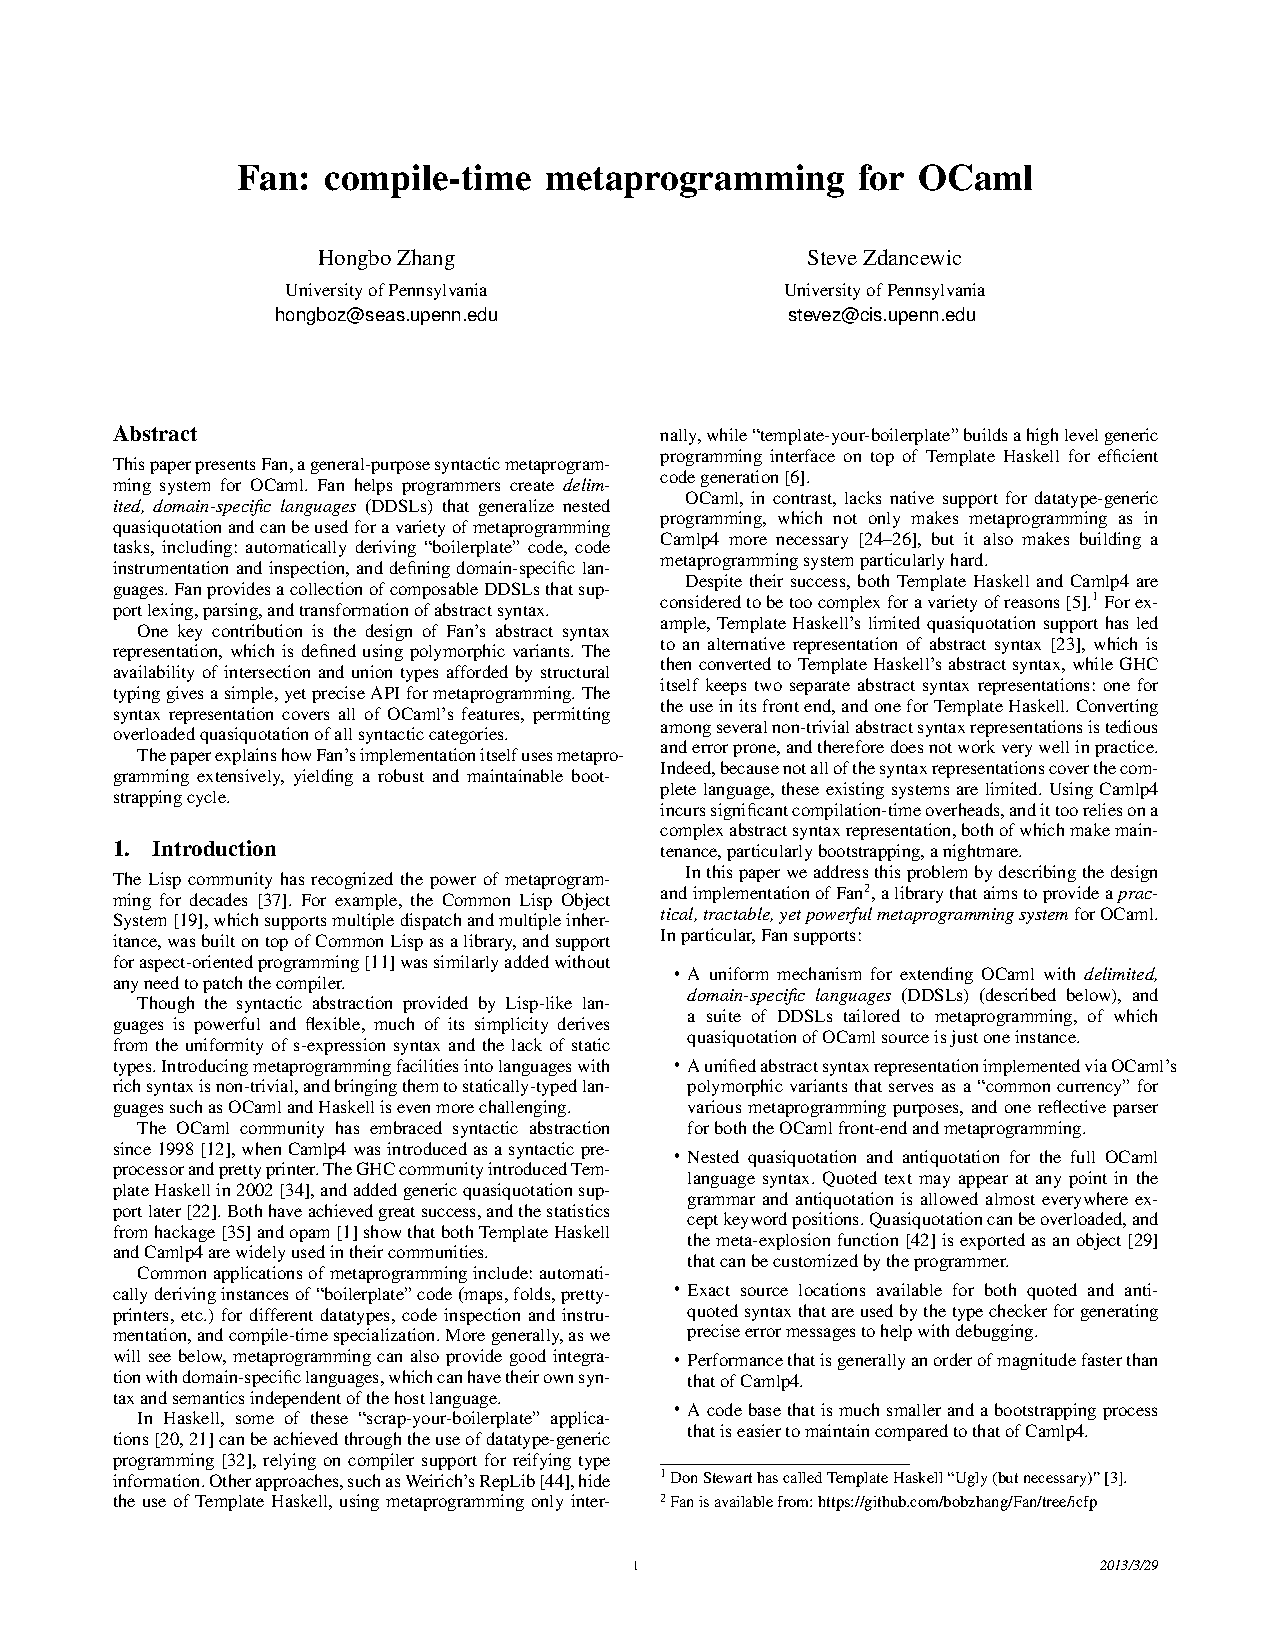
\includegraphics[width=.9\linewidth]{pdf/metaprogramming_for_ocaml.pdf}


\subsection{Fan's quotation system}
\label{sec-5-1}

Fan's metaprogramming has a quotation system \href{http://brion.inria.fr/gallium/index.php/Quotation}{similar to Camlp4}.

The differences lie in serveral following aspects


\subsubsection{Concrete Syntax}
\label{sec-5-1-1}

\begin{itemize}
\item For quotation, Fan uses \verb~{:quot@loc| |}~, while Camlp4 uses \verb~<:quot@< >>~
\item For antiquotation, Fan uses a single \verb~$~ or \verb~$(...)~, while Camlp4 uses \verb~$$~
\item Fan supports nested quasiquotation, while Camlp4 does not.
The following quotation is legal  in Fan.
\begin{verbatim}
{:exp|{:exp| $($x) |}|}
\end{verbatim}
Which is simliar to Common Lisp style macros.
\begin{verbatim}
``(,,x)
\end{verbatim}
\end{itemize}
\subsubsection{Abstract Syntax}
\label{sec-5-1-2}
The definition of Fan's abstract syntax is available here
\url{fansrc/fAst.mli.html}
Fan adopts polymorphic variants for encoding abstract syntax,
there are several major benefits

\begin{itemize}
\item subtyping
For user who wants to reuse part of Fan, the subtyping provides
much more refined types
\item constructor overloading
There's no need to add a prefix for each type
\item polymorphisim
For example, in Fan, to get a location of an ast node, the user
only need to write \verb~loc_of~, without writing \verb~loc_of_exp~,
\verb~loc_of_pat~, \emph{etc.} Other ast processing libraries are also
more generic compared with Camlp4.
\item unqualified, easier to use.
\end{itemize}

The disadvantage:
Error message is sometimes a problem, however, in Fan, the
default quasiquotation will add type annotation automatically for
the user, we have an optional quasiquotation without type
annotations for advanced user.

For example:

\begin{verbatim}
(** with annotations *)
{:exp|3|}
(** after expansion *)
(`Int (_loc, "3") : FAst.exp )
(** without annotations *)
{:exp'|3|}
(** after expansion *)
`Int (_loc, "3")
\end{verbatim}

\begin{enumerate}
\item location handling
\label{sec-5-1-2-1}
From the user's point of view, Fan has two
abstract syntax representations, with or without locations. They
have exactly the same semantics except handling locations. The
abstract syntax without location is derived from abstract syntax
with location.

For example, the definition of \verb~literal~ (see \href{fansrc/fAst.mli.html}{fAst}) are as follows:

\begin{verbatim}
(** literal with locations [FAst]*)
type literal =
  [ `Chr of (loc * string)
  | `Int of (loc * string)
  | `Int32 of (loc * string)
  | `Int64 of (loc * string)
  | `Flo of (loc * string)
  | `Nativeint of (loc * string)
  | `Str of (loc * string)]   


(** literal without locations [FAstN]*)
type literal =
  [ `Chr of string
  | `Int of  string
  | `Int32 of  string
  | `Int64 of string
  | `Flo of string
  | `Nativeint of string
  | `Str of string]
\end{verbatim}
For ast without locations, the naming convention is a \verb~N~ postfix.
Programming abstract syntax without caring about locations is way
more easier. Location is important for debugging and meaningful
error message, however, some scenarios, for example, code
generation, don't need precise location.

There are serveral helpful functions for location handling

\begin{enumerate}
\item \verb~loc_of~
it would fetch location from any type in module FAst
\item Objs.strip\_[type]

For example, Objs.strip\_ctyp would strip the location for
ctyp, their type signature are as follows: (\href{https://github.com/bobzhang/ftop}{ftop} would help!)

\begin{verbatim}
utop $ Objs.strip_case;;
- : FAst.case -> FAstN.case = <fun>
utop $ Objs.strip_exp;;
- : FAst.exp -> FAstN.exp = <fun>
\end{verbatim}
\item FanAstN.fill\_[type]
It's opposite to strip
\begin{verbatim}
utop $ FanAstN.fill_exp;;
- : FLoc.t -> FAstN.exp -> FAst.exp = <fun>
utop $ FanAstN.fill_case;;
- : FLoc.t -> FAstN.case -> FAst.case = <fun>
\end{verbatim}
\end{enumerate}

There is also a suite of quasiquotation for ast without locations.

\begin{verbatim}
(** with annotations, [-] means minus locations *)
{:exp-|3|}
(** after expansion *)
(`Int  "3" : FAstN.exp )

(** without annotations *)
{:exp-'|3|}
(** after expansion *)
`Int  "3"
\end{verbatim}
\end{enumerate}
\subsection{Quotation DDSL}
\label{sec-5-2}

\subsection{Parser DDSL}
\label{sec-5-3}
% Emacs 23.3.50.1 (Org mode 8.0.3)
\end{document}